\PassOptionsToPackage{dvipsnames,table}{xcolor}
\documentclass[10pt]{beamer}
\usetheme[options]{Madrid} 
\usepackage{../../latex/Cours}

\begin{document}
	
	\input{\detokenize{../../latex/MacrosCours.tex}}
	\setcounter{numchap}{10}
	
	\newcommand{\AB}{\cnum Arbres}
	
	\pythonmode

% Relation entre hauteur et taille
\begin{frame}
	\mframe{\AB}
	\begin{alertblock}{Parcours d'un arbre}
		On peut parcourir un arbre binaire :
		\begin{itemize}[label=\textbullet]
			\item<2-> En largeur, cela revient à lister les noeuds par ordre croissant de profondeur et de gauche à droite \\
			      \onslide<3-> \textcolor{gray}{L'implémentation de ce parcours peut se faire à l'aide d'une file dans laquelle on stocke les noeuds restants à parcourir. A chaque fois qu'on traite un noeud, on le defile et on enfile ses fils (voir la fiche d'activité).}
			\item<3-> En profondeur, on tire alors partie de la structure récursive des arbres. Pour parcourir l'arbre $T=(e,sag,sad)$ on doit relancer le parcours sur $sag$ et $sad$. On distingue alors trois parcours suivant que $e$ est affiché avant, entre ou après $sag$ et $sad$ :
			      \begin{itemize}[label=\textbullet]
				      \item<4-> Dans le parcours préfixé, $e$ est affiché avant de parcourir $sag$ et $sad$.
				      \item<5-> Dans le parcours infixé, $e$ est affiché après le parcours de $sag$ mais avant celui de  $sad$.
				      \item<6-> Dans le parcours suffixé, $e$ est affiché après le parcours de $sag$ et $sad$
			      \end{itemize}
		\end{itemize}
	\end{alertblock}
\end{frame}


\begin{frame}
	\mframe{\AB}
	\begin{exampleblock}{Exemple}
		\begin{center}
			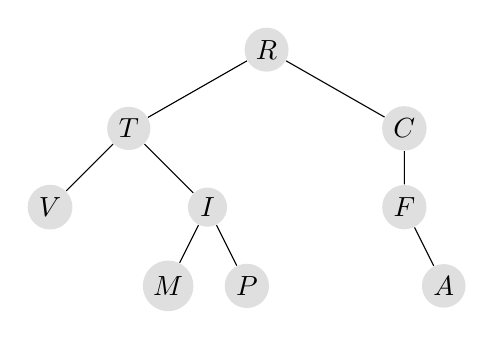
\begin{tikzpicture}[level distance=10mm]
				\tikzstyle{every node}=[fill=gray!25,circle,inner sep=2pt]
				\tikzstyle{level 1}=[sibling distance=35mm,
				set style={{every node}+=[fill=gray!25]}]
				\tikzstyle{level 2}=[sibling distance=20mm,
				set style={{every node}+=[fill=gray!25]}]
				\tikzstyle{level 3}=[sibling distance=10mm,
				set style={{every node}+=[fill=gray!25]}]
				\node {$R$}
				child {node {$T$}
					child {node {$V$}
					}
					child {node {$I$}
						child {node {$M$}}
						child {node {$P$}}
					}
				}
				child {node {$C$}
					child {node {$F$}
						child[fill=none] {edge from parent[draw=none]}
						child {node {$A$}}
					}
				}
				;
			\end{tikzpicture}
	\end{center}
	
		Donner l'ordre des noeuds lorsqu'on parcourt l'arbre ci-dessus :
		\begin{itemize}[label=\textbullet]
			\item<1-> En largeur
			\item<2-> En profondeur préfixé
			\item<3-> En profondeur infixé
			\item<4-> En profondeur suffixé
		\end{itemize}
	\end{exampleblock}
\end{frame}


\end{document}